\section{Multigrid structure}

Let us now move on the structure used to handle the multigrid method. Is it the most important structure to build. If we define our structure in the right way, smoothing, restricting and prolonging are fairly straightforward.

Let us first note that throughout the program, we have two different global node numbering. One for the high degree interpolation, $lnodesP$, and one for the interpolation with $p=1$ used in the multigrid, $lnodes1$. As expalined in the theory chapter, we therefore need functions to transfer the high degree residual from $lnodesP$ to $lnodes1$ and then to transfer the coarse grid correction from $lnodes1$ to $lnodesP$. The details of that transfer are not given here but the implementation from the theory is rather simple. 

We will focus here on the structure we build to handle the multigrid using the global numbering used by $lnodes1$. For each level, we need to know : 

\begin{enumerate}
\item The number of nodes on that level
\item The number of quadrants on that level
\item Which nodes form the $k$-th quadrant
\item If a given quadrant has children on the upper level and if so, which quadrants they are
\item What quadrants are hanging on that level
\item The hanging information of the hanging quadrants
\end{enumerate} 

Several other arrays are also contained in the structure to store the value of the solution at that level, the right-hand side, some geometric factors, ...

Building the structure is a two-step process : we first fill the highest level (corresponding to the finest grid) and then we recursively fill the levels by the information contained in the upper level (we use level $lev+1$ to fill level $lev$).

\subsection{Filling the highest level}

At the highest level, called $maxlev$, it is obvious that the number of nodes, $N^{maxlev}$, is the number of nodes in $lnodes1$, the number of quadrants, $Q^{maxlev}$, is the number of quadrants in the forest and the nodes for the $k$-th quadrant, $nodes^{maxlev}_{i;k}$, are given by $element\_nodes$ in $lnodes1$. There is no upper level so we do not need to care about the children (the array $up^{maxlev}$ is set to -1).

We then have an array containing boolean flags to see if quadrant $k$ has hanging nodes. This is easy to see from the $face\_code$ (see above).

\begin{align*}
hang_k^{maxlev} &= 1 &\text{if quadrant $k$ contains hanging nodes}\\
&= 0 &\text{if quadrant $k$ does not contain hanging nodes} 
\end{align*} 

For quadrants where there is at least one hanging node, we decode the $face\_code$ using the function defined in the previous section and we store the information. 

\begin{align*}
hang\_info^{maxlev}_{i;k} &= -1 &\text{if corner $i$ in quadrant $k$ is not hanging}\\
 &= a &\text{if $a$ is the non hanging corner corresponding to $i$}
\end{align*}

\subsection{Recursively filling the lower levels}

\begin{figure}
\centering
\begin{subfigure}{.5\textwidth}
  \centering
  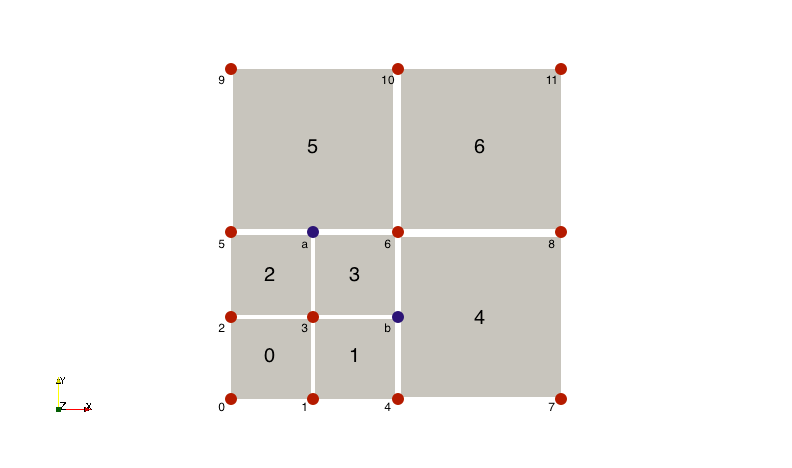
\includegraphics[width=1.2\linewidth]{Implementation/multi_ex_2.png}
  \caption{Mesh at level 2}
  \label{multi_ex_2}
\end{subfigure}%
\begin{subfigure}{.5\textwidth}
  \centering
  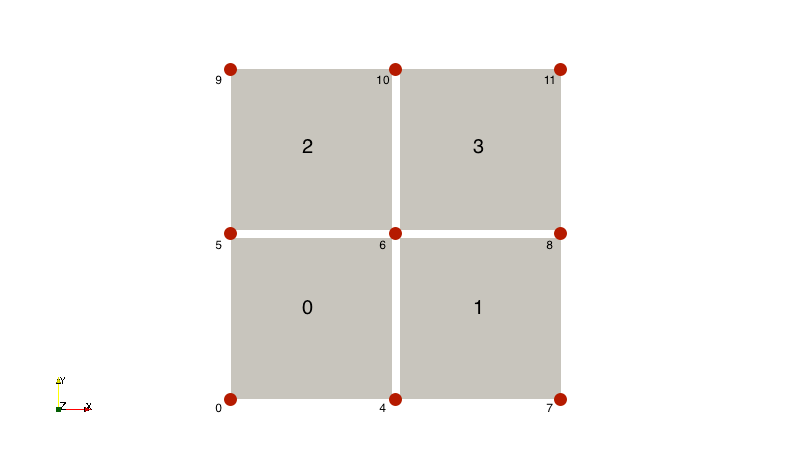
\includegraphics[width=1.2\linewidth]{Implementation/multi_ex_1.png}
  \caption{Mesh at level 1}
  \label{multi_ex_1}
\end{subfigure}
\caption{Example of two meshes at level 1 and 2. We can see that when we go from level 2 to level 1, all quadrants that had a refinement level of 2 are replaced by their parent. Moreover, the parent of the quadrants with level of refinement 2 that were hanging at level 2 is not hanging at level 1. The global nodes are in red (with their global number) and the hanging nodes in blue. The global number of the quadrants is also given.}
\label{multi_ex}
\end{figure}

Let us remember that the mesh at level $lev$ is the mesh at level $lev+1$ where all quadrants with level of refinement $lev+1$ have been replaced by their parent. We can see an example in figure \ref{multi_ex}. At level 1, all quadrants with level 2 have been replaced by their parent.

An important thing to note here is that if a quadrant with level of refinement $lev+1$ is hanging at level $lev+1$, then the corresponding parent at level $lev$ is not hanging. This is a direct consequence of the fact that two neighboring quadrants differ by at most one level in their refinement levels. In the example in figure \ref{multi_ex}, we can indeed see that the parent of the quadrants that were hanging at level 2 is not hanging at level 1.

The first thing to do is to compute the number of quadrants at level $lev$. If, at level $lev+1$, there are $q^{lev+1}$ quadrants with a level of refinement of $lev+1$, then it is given by : 

$$Q^{lev} = Q^{lev+1} - \frac{3}{4} q^{lev+1}$$

Then, we go quadrant by quadrant following their global ordering (given by the space-filling curve). If the current quadrant has a refinement level inferior or equal to $lev$, then we copy the information from level $lev+1$ to level $lev$. However, if we reach a quadrant with a refinement level of $lev+1$, then we have to coarsen. An important thing to note is that, if we visit the quadrants in their global order given by the space filling curve, then the four quadrants we have to replace by their parent when we coarsen are always positioned consecutively. Therefore, we can fill the $up$ array easily. For the example in figure \ref{multi_ex}, we have :

$$up^1_0 = \begin{bmatrix}
0 & 1 & 2 & 3
\end{bmatrix}$$

The $up$ array for the other quadrants are filled with -1 since they do not have children. We can also use the fact that the children are placed consecutively and the fact that when we coarsen we are sure that no node is hanging to easily fill the $nodes$ array. In our example this yields : 

\begin{align*}
nodes^1_0 &= \begin{bmatrix}
nodes^2_{0;0} & nodes^2_{1;1} & nodes^2_{2;2} & nodes^2_{3;3}
\end{bmatrix}\\
&= \begin{bmatrix}
0 & 4 & 5 & 6
\end{bmatrix}
\end{align*}

The last thing to handle for that set of quadrants is the hanging information. Since we coarsen, the parent is not hanging. In our example, that just means setting $hang^1_0 = 0$. 

After having gone through all the quadrants, we still need to compute the number of global nodes at level $lev$. The idea is to fill an array with all the nodes we see when we go through the quadrants (which is therefore of length $4Q^{lev}$), then to sort this array and count the number of different global nodes we have. That also allows us to set up a mapping between the numbering of the nodes at level $lev$ and the global numbering given in $lnodes1$. That mapping is very useful when we have to perform an operation on the nodes at a given level (for example, during the smoothing). 
 
Let us finally say that the minimum level ($lev = 0$) is the macro-mesh. It is a conforming mesh and on it, we solve the linear system of equation exactly using the Lapack library (see \cite{lapack} for information).  
 












